% !TEX root = ../../../main.tex
% 来源：中学数学实验教材·第三册（高中数学）
% 章节：不等式和解不等式 / 解不等式
% 原始文件：3.tex，行 1661-1681
% 类型：tikz
% ---
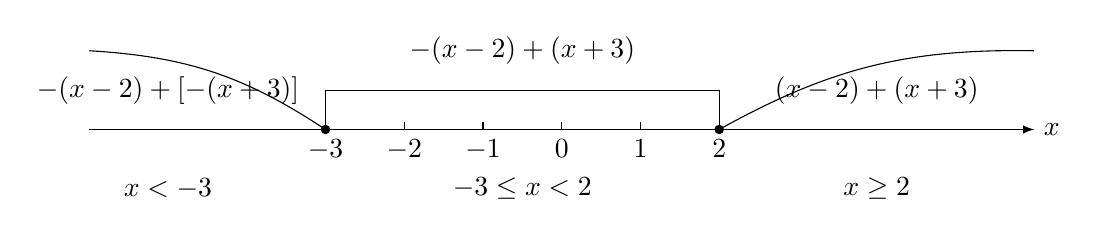
\begin{tikzpicture}[>=latex]
\draw[->] (-6,0)--(6,0)node[right]{$x$};
\foreach \x in {-3,-2,...,2}
{
    \draw (\x,0)node[below]{$\x$}--(\x,.1);
}
\draw (-3,0) [fill=black] circle(1.5pt);
\draw (2,0) [fill=black]circle (1.5pt);

\draw (-3,0)--(-3,.5)--(2,.5)--(2,0);
\draw (-6,1)to [bend left=15] (-3,0);
\draw (6,1)to [bend left=-15] (2,0);

\node at (-5,-.75){$x<-3$}; 
\node at (-.5,-.75){$-3\le x<2$};
\node at (4,-.75){$x\ge 2$};

\node at (-5,.5){$-(x-2)+[-(x+3)]$}; 
\node at (-.5,1){$-(x-2)+(x+3)$};
\node at (4,.5){$(x-2)+(x+3)$};
\end{tikzpicture}
